% The following is for LaTeX2e.
\documentclass[10pt]{article}
\usepackage{samplesty} % Includes the sample style file
\usepackage{epsfig}

% For algorithm elements
\usepackage{algorithm}
\usepackage[noend]{algpseudocode}

%For Neural Network Diagram
\usepackage{tikz}
\usetikzlibrary{positioning}


% The following is for LaTeX 2.09.
% \documentstyle[11pt,twocolumn,samplesty,epsfig]{article}

\begin{document}

\title{An approach to 2D/3D registration using deep reinforcement learning \\(ACDDE 2017)}

\author{Eungjune Shim, \\
Center for Bionics, Korea Institute of Science and Technology, \\
Department of Biomedical Engineering, University of Science and Technology, Seoul, Korea
\and Youngjun Kim\thanks{Corresponding author email: junekim@kist.re.kr},
\\ Center for Bionics, Korea Institute of Science and Technology, Seoul, Korea}


%

\date{2017-05}
\maketitle

\begin{abstract}
 Deep Q Learning method is a novel approach to approximate value functions of reinforcement learning. This has been successfully applied to solve problems such as robot control, elevator scheduling, telecommunication networks. We applied this method to a simplified 2D-3D registration problem; Point-based visual servoing simulator. The simulator environment has been virtually organized in three-dimensional space: four three-dimensional target point vectors and two-dimensional correct point vector, and a virtual camera are defined. For each timesteps, camera moves according to the output of a neural network(Q-network), and the 3D target points are projected onto the viewport. The purpose of this simulator is to reduce 2D vector error between target and correct point vectors. The Q-network takes states of current timestep, decide a action, receive rewards and update weights. The actins are defined in six: camera moves forward, backward, top, bottom, right, left. The state is defined as four 2D error vectors. As learning processes, the network moves camera with higher possibility of reducing errors. When using well-trained network, there are several benefits compare to conventional methods, such as random searching algorithms or jacobian matrix estimation. While conventional method requires computation of error variance or matrix inverse in every timestep, our proposed method only requires simple network forwarding to find its solution. Since this method used too much simplified registration environment and camera actions, the performance looks a little bit awkward, but there still are a lot to improve from this approach. Firstly, we can define each step's state with much more complex and sophisticated form by replacing the neural network. There are many Convolutional Neural Networks(CNNs) proposed to handle 2D images, the state can be defined simply using virtual camera's rendered image, not eight-digit 2D point error vectors. Secondly, the camera actions can be more natural and efficient by using the whole output possibility of the network, and combining action. As our proposed method shows considerable benefit over the conventional method, the future work from this approach can be expected to be applicable to real 2D-3D registration works.

\vspace*{5mm}
\noindent
{\bf Key words:}  Deep Q Learning, Reinforcement Learning, 2D-3D Registration, Visual Servoing
\end{abstract}

\section{Introduction}

 Deep Q Learning(DQN) method is a novel approach that has been successfully applied to solve problems such as robot control, elevator scheduling, telecomunication networks.

 (Some Related Works)

 We applied this method in a simple point-based virtual visual servoing simulator.

 In the simulator, we use four 2D vector errors to find 3D camera transformation, This is a basic concept of 2D-3D registration, so this approach shows possibility to extend solving 2D-3D registration problems using DQN.


\section{Methods}
Virtual point-based servoing simulator is composed of a camera and a plane containing four circles on it in a virtual 3D space. The plane normal and the camera view vectors are parallel to world coordinate's Y-axis. Since no rotation is possible in the condition of this simulator, camera view vector will not be changed. Normally in visual servoing, four point features are extracted from the rendered image by using image processing algorithms. Since our purpose is to test our DQN-based 2D-3D registration algorithm, we decided to skip this process. Instead of that, we pre-defined the 3D positions of four feature points, extract to the 2D rendering viewport by unproject them. This has the same effect as feature detection. This simulator runs on web browser, used javascript-based \emph{WebGL} library named \emph{Three.js}.

\begin{figure}[htb]
\begin{center}
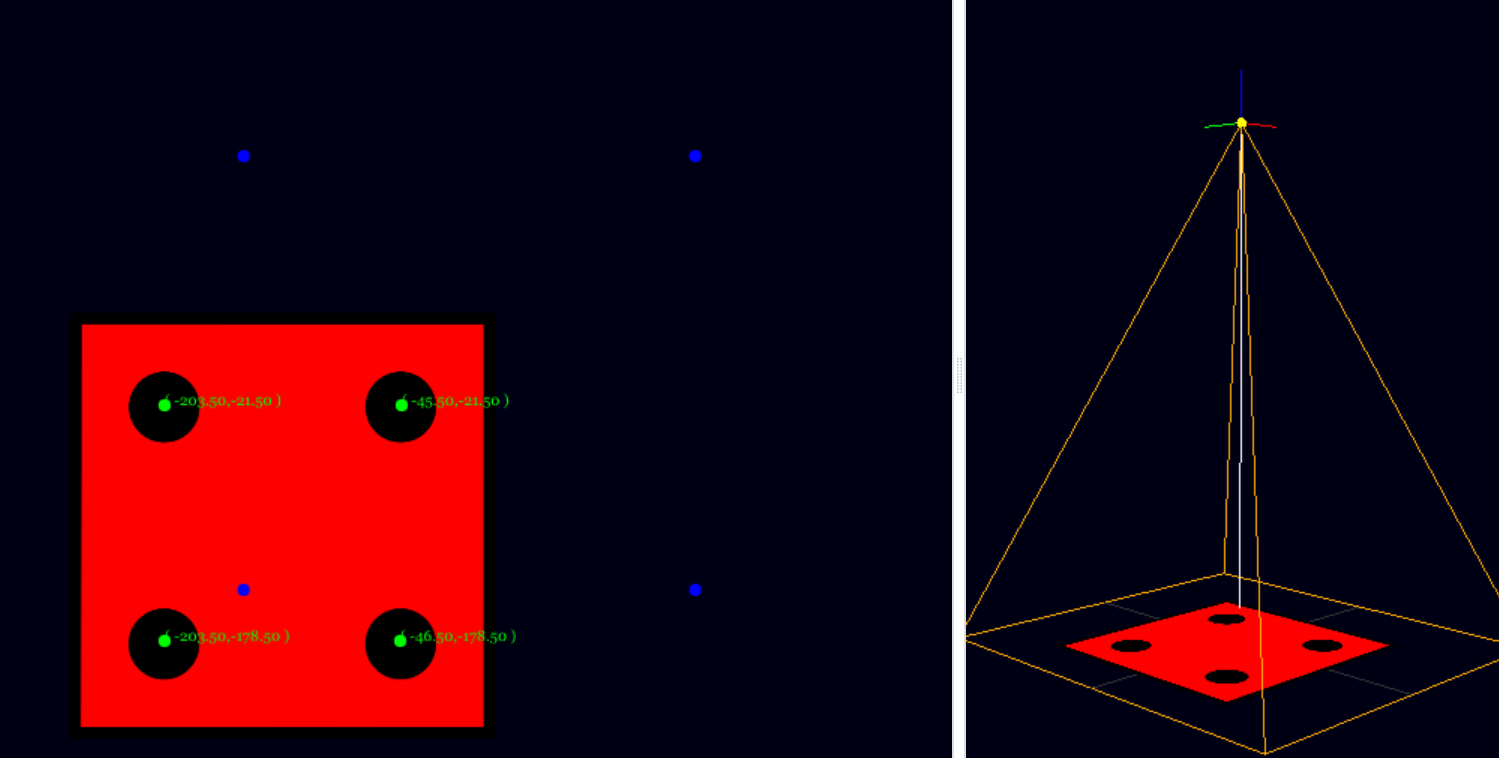
\includegraphics[width=0.8\columnwidth]{images/fig-temp1.png}
\caption{3D Servoing Environment, renderer image(left), and 3D objects(right)}
\label{fig1}
\end{center}
\end{figure}

DQN training is based on Q-learning\cite{ref1} algorithm, using Q-network for approximating Q-table. Experience replay and target $Q$ are also applied to our method to prevent divergence and  stablize the process. For every timestep $t$, environment $\varepsilon$, composed of states$s_t$ actions $a_t$, and rewards $r_t$ are defined. The agent of DQN has Q-network \ref{actions}, predicts rewards of each action values, so user-defined reward can backpropagate and update weight inside the network\cite{ref2}. In our proposed method, we simply set the state as four error vectors of 2D target points and corresponding ground-truth points. The reward is given according to the variance of error vector size. If the total amount of the error is decreased in $x_{t+1}$, the agent receives reward of value $1.0$, and if the error is increased, the reward is $-1.0$. The total experience size of sequence is set to $30000$ and the training task proceeds when $size(\epsilon) \geq 100$. The action $a$ are consist of six actions as mentioned: forward, backward, up, down, right, left. For each actions, all the distance the camera move is set to $1$. The agent interacts with the simulator by selecting actions in a way that maximises future rewards. The Q-network is composed of a simple four-layered neural network: input layer, two fully-connected layers with 50 neurons, and regression output layer Fig. ~\ref{fig2}.

\begin{equation}\label{actions}
  Q(s, a) \Rightarrow r
\end{equation}


\tikzset{%
  every neuron/.style={
    circle,
    draw,
    minimum size=1cm
  },
  neuron missing/.style={
    draw=none,
    scale=4,
    text height=0.333cm,
    execute at begin node=\color{black}$\vdots$
  },
}
\begin{figure}[htb]
\begin{center}
  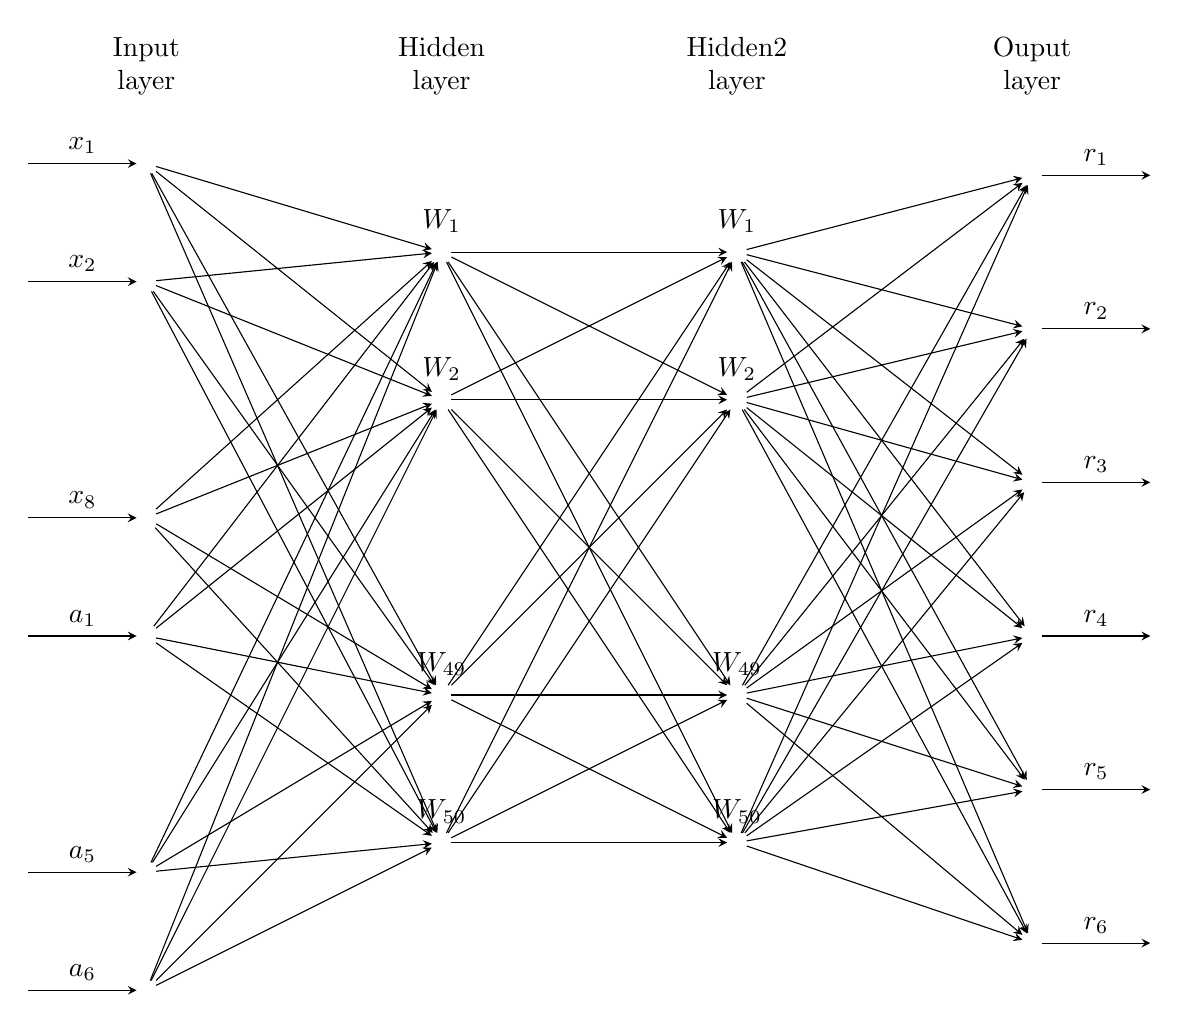
\begin{tikzpicture}[x=1.5cm, y=1.5cm, >=stealth]

 \def\layersep{2.5}
 %Input Layer
  \foreach \m/\l [count=\y] in {1,2,missing,3,4,missing,5,6}
    \node [every neuron/.try, neuron \m/.try] (input-\m) at (0*\layersep,2.5-\y) {};

%Hidden Layer 1
  \foreach \m [count=\y] in {1,2,missing,3,4}
    \node [every neuron/.try, neuron \m/.try ] (hidden-\m) at (1*\layersep,2-\y*1.25) {};

%Hidden Layer 2
  \foreach \m [count=\y] in {1,2,missing,3,4}
    \node [every neuron/.try, neuron \m/.try ] (hidden2-\m) at (2*\layersep,2-\y*1.25) {};
%Hidden Layer 1
  \foreach \m [count=\y] in {1,...,6}
    \node [every neuron/.try, neuron \m/.try ] (output-\m) at (3*\layersep,2.7-\y*1.3) {};



  \foreach \l [count=\i] in {1,2,8,1,5,6}
  {
    \ifthenelse{\i < 4}{\draw [<-] (input-\i) -- ++(-1,0) node [above, midway] {$x_{\l}$};}{\draw [<-] (input-\i) -- ++(-1,0) node [above, midway] {$a_{\l}$};}

  }


  \foreach \l [count=\i] in {1,2,49,50}
    \node [above] at (hidden-\i.north) {$W_{\l}$};

  \foreach \l [count=\i] in {1,2,49,50}
    \node [above] at (hidden2-\i.north) {$W_{\l}$};


  %Append Edge
  \foreach \l [count=\i] in {1,...,6}
    \draw [->] (output-\i) -- ++(1,0)
      node [above, midway] {$r_{\l}$};

  \foreach \i in {1,...,6}
    \foreach \j in {1,...,4}
      \draw [->] (input-\i) -- (hidden-\j);

  \foreach \i in {1,...,4}
    \foreach \j in {1,...,4}
      \draw [->] (hidden-\i) -- (hidden2-\j);

  \foreach \i in {1,...,4}
    \foreach \j in {1,...,6}
      \draw [->] (hidden2-\i) -- (output-\j);

  \foreach \l [count=\x from 0] in {Input, Hidden, Hidden2, Ouput}
    \node [align=center, above] at (\x*\layersep,2) {\l \\ layer};

  \end{tikzpicture}
\caption{Q-network in the agent. Input layer is composed of states $s$ and actions $a$. The output layer is rewards}
\label{fig2}
\end{center}
\end{figure}

In the training process, camera position is initialized randomly where all four target feature points are visible. If the error value variation $E_t$ between $x_{t+1}$ and $x_t$ is less than $10.0$ the camera is repositioned according to the camera position initialization function. After $100$ experiences are stacked, the training starts. The agent takes the state $x_t$ and decide action according to DQN network policy; As learning progresses, agent relies more on Q-network then randomly select in order to choose action. The camera performs the action specified by the agent ($camera.GoTo(a_t)$). The reward $r_t$ is fixed according to $E_t$, and the agent takes reward and updates weights of Q-network ($agent.Backward(r_t)$).

 \begin{algorithm}
   \caption{DQN training process for point-based visual servoing}\label{algo1}
   \begin{algorithmic}[1]

     \State camera.RandomPosition()


     \For {$t$ in $T$}

     \State $a_t$ =  argmax(Q(s, a;$\theta$))
     \State camera.GoTo($a_t$)
     \State $E_t$ = Error($x_{t+1}$) - Error($x_t$)
     \If {E $\geq$ 0}
     \State $r_t$ = $1.0$
     \Else
     \State $r_t$ = -$1.0$
     \EndIf

     agent.Backward($r_t$)
     \If{$r_t$ $leq$ 10.0}
     camera.RandomPosition()
     \EndIf

     \EndFor

   \end{algorithmic}
 \end{algorithm}


\section{Results}
(Some Pictures)

(Graph during training)



\section{Discussion}
 Our proposed DQN model is trained using 2D feature vector error as the environment $\varepsilon$, decided correct action $a$ for servoing virtual camera in 3D space. Under our DQN policy, the model became totally dependent the Q-network deciding action after ??????? steps. From this point, the network is well-trained as far as possible, so further training is meaningless. This well-trained model can conduct registration from a random position to the optimal position within average of ??? seconds. The visualized camera moved smoothly with almost no unnecessary movement. Compare to conventional method, such as random tree searching algorithm or jacobian matrix estimation, our proposed method has several benefits. First, the amount of calculation is greatly reduced while conventional method requires large amount of computations. Both methods requires calculation of error varation in every timestep. Furthermore, jacobian matrix estimation method requires to calculate inverse (or pseudoinverse) matrix everytime. In random searching algorithm, such as simulated annealing can easily to fall into local minima, and also, there are too much unnecessary movement durign registration. The DQN method requires such calculation only when it is being trained. Once training task is done, this does not require any complex computation, and shows efficient servoing movement. Second, the proposed method is very easy to implement. Once the form of the network, environment, actions, rewards and some parameters are configured, no more difficult tasks are needed except waiting the agent to be trained.

 For now, there are several limitations that need to be improved. Firstly, Camera movement is somewhat inefficient like staircase. Because the direction and range in which camera can move is fixed in six actions. The jacobian matrix estimation method can put out all-round 3D translation and rotation vector, this method currently shows much smoother motion during registration. Since all the distance the camera move is $1$, it is also inefficient in terms of utilization of error sizes. Secondly, states $x_t$ is too simple to apply to real 2D-3D registrations. Our current method defined $x_t$ as four 2D point vector errors, but real 2D-3D registration, larger and much more complex features need to be used to define current state.

  Most of this limitations can soon be resolved in the future works. The camera movement problem can be solved by combining actions. Instead of choosing a single action predicted by $argmax(Q(s, a; \theta ))$, we can use the whole values in output layer of Q-network, and add the action vectors multiplied by the corresponding predicted reward values. This can give a much higher degree of freedom(DOF) to camera motion. Also, adding rotation action is necessary to perform complicated 2D-3D registration. More sophisticated form of stats $x$ can also be easily defined. This is the greatest potential and advantage of using DQN rather then other methods; Comparing jacobian matrix estimation method, as the feature of input state gets more complicated, the computation and complexity for deciding proper action gets exponentially more difficult.
  This method can use CNN that can self-study the feature information of input images, this method is extreamly easy to implement, and also, can expect good results. There already are many DQN methods succesfully applied to play games that uses rendered game images as input state, deep CNN as its Q-networks\cite{ref2}. Setting stochastic reward can also efficiently utilizes the size of error variation, and reduces registraiton time. To sum it up, our future DQN model uses deep CNN for its value network. takes rendered image of each timestep as input state, predicts actions, and perform registration by combining whole output Q-network layer.



\section{Conclusion}

We have proposed and developed a DQN method for 2D-3D registartion. This method is successfuly applied to optimize and solve the point-based visual servoing simulator. This simulator takes 2D feature states to perform in 3D, this basically can be regarded as very simplified 2D-3D registration simulator. Although this is simplified problem, the proposed approach has its strength in terms of solving similar but more complex problems compare to conventional registration methods; For example, jacobian matrix estimation method requires exponential computation and high difficulty as the problem becomes more complicated. Also, most of searching algorithm such as simulated annealing, heel climbing methods for optimizing 2D-3D registration requires to calculate the similarity of two states, and the complexity of two states gets higher, the amount of computation also gets larger. While the DQN only forwards input states to the network, once it is well-trained.


\section*{Acknowledgement}
This research was supported by the KIST institutional program (??????, ???????).


\bibliographystyle{elsarticle-num}
\bibliography{references}

%
% \begin{thebibliography}{9}
% \bibitem{ref1}
% S.~Fortune, A sweepline algorithm for Voronoi diagrams,
% {\it Algorithmica} {\bf 2} (1987), pp.153--174.
%
% \bibitem{ref2}
% G.~Farin, {\it Curves and Surfaces for Computer Aided Geometric
% Design: A Practical Guide}, Academic Press, San Diego, 1988.
%
% \bibitem{ref3}
% A. Okabe, B. Boots, K. Sugihara, and S.N. Chiu,
% {\it Spatial Tessellations: Concepts and Applications of
% Voronoi Diagrams}, 2nd Edition, John Wiles \& Sons, Chichester, 2000.
%
% \bibitem{ref4}
% T. Pavlidis, Curve fitting with conic splines,
% {\it ACM Transactions on Graphics} {\bf 19} (1983), pp. 151--159.
%
% \bibitem{ref5}
% K. Sugihara's Homepage,
% \texttt{http://www.simplex.t.u-tokyo.ac.jp/\~{}sugihara/}, 2005.
%
% \bibitem{ref6}
% G. Taubin, A signal processing approach to fair surface design,
% in {\it Proc. of SIGGRAPH} (1995), pp. 351--358.
%
% \end{thebibliography}

\end{document}
